\setcounter{page}{1}
\section*{Zielsetzung}
Mit dem Versuch soll der Hall-Effekt durch Messung der
Hall-Spannung experimentell untersucht werden. %untersucht

\section{Theorie}

\subsection{Elektrische Leitfähigkeit}
Jeder Festkörper besitzt nach der Quantenmechanik und dem Pauli-Prinzip
Energiebänder.
Diese geben die für ein gebundenes Elektron möglichen Energiebereiche an. Auf den Bändern bzw. Valenzbänder kann das Elektron weder
Energie aufnehmen noch abgeben.
Es kann also nicht beschleunigen bzw. abbremsen (z. B. durch ein äußeres E-Feld).
Erst auf den sogennanten Leitungsbändern ist es für das Elektron möglich
sich frei zu bewegen.
Lediglich bei leitenden Elementen (z. B. Metallen) ist der Abstand zwischen Valenzband und \emph{Leitfähigkeitsband} gering genug, sodass die Elektron das Band
wechseln können.
Bei Isolatoren befinden sich keine freien Elektronen auf dem \emph{Leitfähigkeitsband}.
In Metallen kommt es zu Bildung von Gitterstrukturen.
Auf diesen verhalten sich die \emph{Leitungselektronen}, wie Teilchen eines idealen Gases.
Es es kommt unter den Elektronen zu Stoßvorgängen.
Die gemittelte Zeit zwischen zwei Stößen wird als \emph{mittlere Flugzeit} $\overline{\tau}$ bezeichnet.

Wird ein Elektron mittels $\vec{F}=\map{e}\vec{E}$ ($\map{e}\, \hat{=}$ Elementarladung) beschleunigt, %Komma
ergibt sich für die \emph{Driftgeschwindigkeit}: %die

\begin{equation}
\label{eq:drift_v}
\vec{\overline{v}}\ua{d}=\frac{1}{2}\Delta\vec{v}=-\frac{1}{2}\frac{\map{e}}{\map{m}\ua{e}}\vec{E}\,\overline{\tau}
\end{equation}

Hierbei sei $\map{m}\ua{e}$ die Elektronenmasse.
Mittels der \emph{Driftgeschwindigkeit} kann nun auf die Stromdichte $j$ geschlossen werden. Dazu:

\begin{align}
j&=-n\overline{v}\ua{d}\map{e}=\frac{1}{2}\frac{\map{e^2}}{\map{m}\ua{e}}n E\overline{\tau}\notag \\
\Leftrightarrow \quad \overline{v}\ua{d}&=\frac{j}{n\map{e}}\label{eq:stromdicht}
\end{align}
Die Größe $n$ gibt die Anzahl der Elektronen pro Volumeneinheit an.
Mit der idealisierten Annahme eines homogenen Leiters, können %wort zu viel
$j=\frac{I}{Q}$ und $E=\frac{U}{L}$ umgeschrieben werden.
Dabei sei $Q$ der Querschnitt und $L$ die Länge des Leiters.
Mittels dem ohmschen Gesetz folgt anschließend

\begin{equation}
\label{eq:wider}
R=2\frac{\map{m}\ua{e}}{\map{e}^2}\frac{1}{n\overline{\tau}}\frac{L}{Q}
\end{equation}

\subsection{Der Hall-Effekt}
Der \emph{Hall-Effekt} kommt immer dann zu Stande, wenn %zustande oder zu Stande
ein Magnetfeld auf einer stromdruchflossene %muss nicht senkrecht stehen, damit der zustande kommt
Leiterplatte (Dicke $d$ und Breite $b$) wirkt.
Die Lorentzkraft $\vec{F}\ua{l}$ sorgt für eine Ablenkung der Elektronen.
Die Ablenkung bewirkt eine Potentialdifferenz zwischen den
Punkten $A$ und $B$ (vgl. \ref{fig: auf_hall}). Dadruch entsteht gleichzeitig ein %ref
weiteres elektrisches Feld $E\ua{y}$, das der Elektronenbewegung entgegen wirkt. %elektrisches Feld, das der Elektronenbewegung entgegen wirkt
Die Spannung zwischen $A$ und $B$ wächst so lange an, bis es zu einem Kräftegleichgewicht zwischen der Lorentz- und Coulombkraft kommt.
Für die Hallspannung kann dan gefolgert werden mit%stil

\begin{equation}
\label{eq:hall_span}
U\ua{H}=E\ua{y}b=\overline{v}\ua{d}Bd=-\frac{1}{n\map{e}}\frac{BI\ua{q}}{d}.
\end{equation}
Die Hallspannung kann also Auskunft über die Ladungsträgerdichte $n$ geben.
Die Gleichung \eqref{eq:hall_span} ist bei konstanter Stromstärke eine Geradengleichung der Form $U\ua{H}=mB$ mit %anderen Fall berücksichtigen
\begin{align}
m&=\frac{1}{n\map{e}}\frac{I\ua{q}}{d} \notag \\
\Leftrightarrow \quad n&=\frac{I\ua{q}}{m\map{e}d}\label{eq:steig_teil_anz}
\end{align}

Lässt man das Magnetfeld konstant so ergibt sich $U\ua{H}=mI$ mit
\begin{align}
m&=\frac{1}{n\map{e}}\frac{B\ua{q}}{d} \notag \\
\Leftrightarrow \quad n&=\frac{B\ua{q}}{m\map{e}d}\label{eq:steig_teil_anz_konstb}
\end{align}


\subsection{Berechnung mikroskopischer Leitfähigkeitsparameter}
Mithilfe des Widerstandes und der \emph{Hall-Spannung} kann nun auf
einige mikroskopische Leitfähigkeitsparameter geschlossen werden.
Zum einen lässt sich die mittlere \emph{freie Weglänge} $\overline{l}$ bestimmen.
Dazu wird der Zusammenhang

\begin{equation*}
\label{eq:freie_weg}
\overline{l}=\overline{\tau}\left|\,v\,\right|
\end{equation*}
verwendet.
Mit $\left|\,v\,\right|$ wird die Totalgeschwindigkeit des Elektrons bezeichnet.
Sie entsteht durch die Wärmebewegung der Kristallbausteine.
Um die Totalgeschwindigkeit eines Elektrons zu bestimmen, nutzt
man die \emph{Fermi-Energie} $E\ua{F}$. Sie spiegelt den Wert des energiereichsten Elektrons am absoluten Nullpunkt wieder.
Und wird mit dem Zusammenhang %wird

\begin{equation}
\label{eq:fermi_e}
E\ua{f}=\frac{h^2}{2\map{m}\ua{e}}\left[\left(\frac{3}{8\pi}\right)^2\right]^{\frac{1}{3}}
\end{equation}
berechnet. In Formel \eqref{eq:fermi_e} wird das Plancksches Wirkungsquantum $h$ benutzt.
Da kaum ein Elektron $E\ua{f}$ erreicht und somit im Wesentlichen nicht
für die elektrische Leitfähigkeit verantwortlich ist, %komma
kann die Totalgeschwindigkeit abgeschätzt werden mit % - komma

\begin{equation}
\label{eq:total_v}
\left|\,\overline{v}\,\right|\approx\left(\frac{2E\ua{F}}{\map{m}\ua{e}}\right)^{\frac{1}{2}}.
\end{equation}
Damit erhalten wir für die  mittlere \emph{freie Weglänge}:
\begin{equation}
\label{eq:mit_frei_weg}
\overline{l}\approx\overline{\tau}\sqrt{\frac{2E\ua{f}}{m\ua{e}}}
\end{equation}

Mittels der Flugzeit $\ov{\tau}$ wird die \emph{Beweglichkeit} $\mu$ errechnet.
Hierzu wird  %stil

\begin{align}
\vec{\ov{v}}\ua{d}&=\mu\vec{E} \notag \\
\Leftrightarrow \quad \mu&=\frac{1}{2}\frac{\map{e}}{m\ua{e}} \label{eq:beweg}
\end{align}
genutzt.

\subsection{Hysterese}

Die \emph{Hysterese} beschreibt in diesem Fall die nicht lineare
Abhängigkeit der magnetischen Flussdichte $B$ zu der
Stromstärke $I$.
In Abbildung \ref{fig: hyste} ist beispielhaft eine Hysteresekurve für die Abhängigkeit
von $B$ zu $H$ zu sehen. An dieser soll der Effekt der Hystere erläutert werden.
Weiter ist bei dem Versuch die sogenannte Remanenz zu beachten (in \ref{fig: hyste} Punkt $\map{P}_2$). %Punkt P2
Sie steht für den Verbleib einer Remanenz-Flussdichte bei $I=0$ (Restmagnetisierung). %heißt das Remanent-Flussdichte?
Nur durch ein ausreichend großes Gegenfeld kann diese beseitigt werden. %ein
Die von der Hysteresekurve eingeschlossene Fläche gibt die für die Magnetisierung benötigte
Arbeit an. Das Aufbringen der Energie sorgt, aber gleichzeitig für eine Erwärmung des Kernes. %letzter Satz notwendig?

\begin{figure}
  \centering
  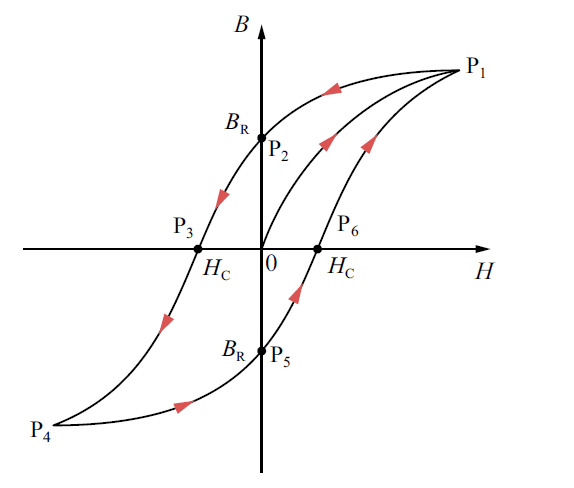
\includegraphics[width=0.5\textwidth]{pics/hystereskurve.png}
  \caption{Hysteresekurve. \cite{hyste}}
  \label{fig: hyste}
\end{figure}
